\documentclass[tikz,border=5pt]{standalone}
\usepackage[T1]{fontenc}
\usepackage{lmodern,amsmath,amssymb}
\usetikzlibrary{arrows.meta,calc,positioning,fit,backgrounds,shapes.geometric,matrix,decorations.pathreplacing,patterns}
\definecolor{ink}{gray}{0.08}
\definecolor{wash}{gray}{0.965}
\definecolor{soft}{gray}{0.45}
\tikzset{box/.style={draw=ink,line width=.65pt,fill=white,align=center,inner sep=4pt,outer sep=0pt,font=\small},flow/.style={draw=ink,line width=.65pt,-{Latex[length=1.8mm,width=1.3mm]},rounded corners=2pt},annotation/.style={font=\scriptsize,text=soft,align=center},groupbox/.style={draw=soft,dashed,line width=.45pt,fill=wash}}
\begin{document}
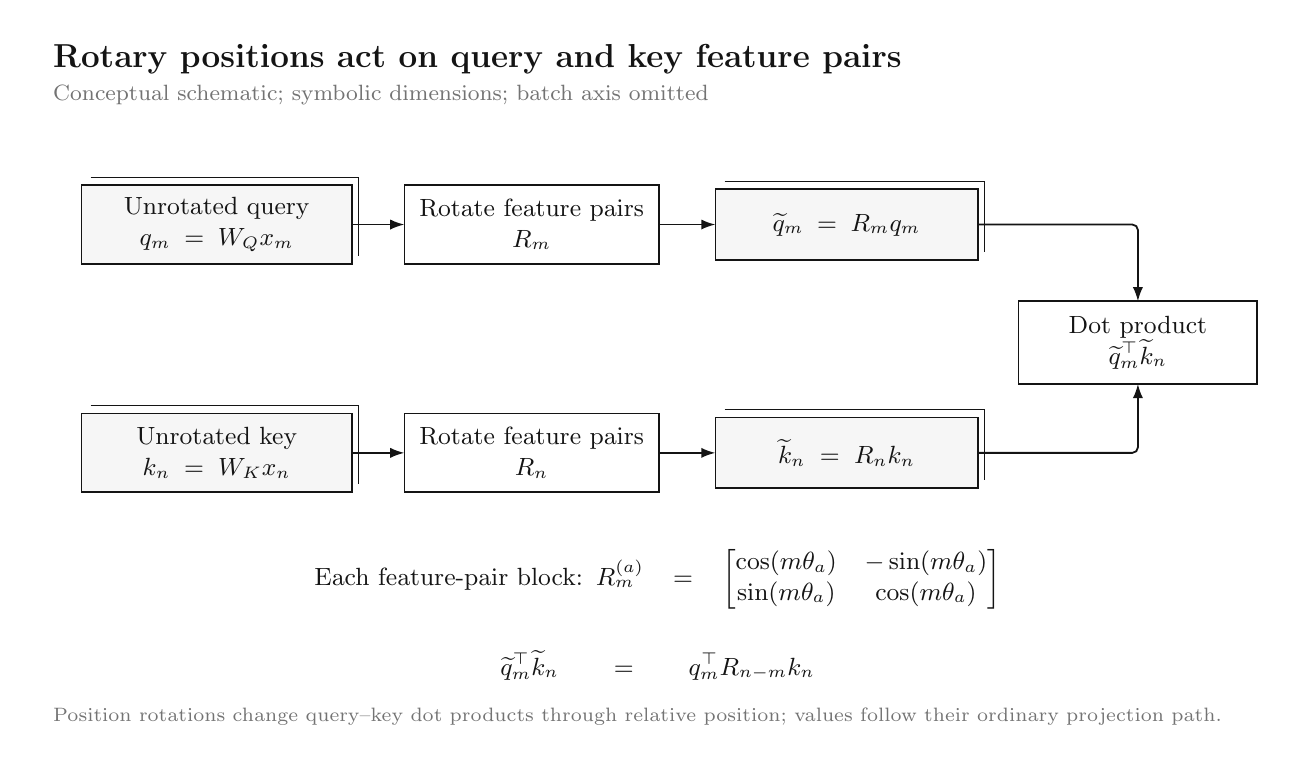
\begin{tikzpicture}[x=1cm,y=-1cm,font=\rmfamily,text=ink]

\path[use as bounding box] (0,0) rectangle (16,9);
\node[anchor=west,font=\large\bfseries] at (.2,.4) {Rotary positions act on query and key feature pairs};
\node[anchor=west,font=\footnotesize,text=soft] at (.2,.85) {Conceptual schematic; symbolic dimensions; batch axis omitted};
\begin{pgfonlayer}{background}
\end{pgfonlayer}
\node[box,fill=wash,minimum width=3.4cm,minimum height=1.0cm,text width=3.15cm] (q) at (2.4,2.5) {Unrotated query\\$q_m=W_Qx_m$};
\draw[ink,line width=.4pt] (0.7999999999999999,1.9) -- (4.199999999999999,1.9) -- (4.199999999999999,2.9);
\node[box,fill=wash,minimum width=3.4cm,minimum height=1.0cm,text width=3.15cm] (k) at (2.4,5.4) {Unrotated key\\$k_n=W_Kx_n$};
\draw[ink,line width=.4pt] (0.7999999999999999,4.800000000000001) -- (4.199999999999999,4.800000000000001) -- (4.199999999999999,5.800000000000001);
\node[box,minimum width=3.2cm,minimum height=1.0cm,text width=2.95cm] (rq) at (6.4,2.5) {Rotate feature pairs\\$R_m$};
\node[box,minimum width=3.2cm,minimum height=1.0cm,text width=2.95cm] (rk) at (6.4,5.4) {Rotate feature pairs\\$R_n$};
\node[box,fill=wash,minimum width=3.3cm,minimum height=0.9cm,text width=3.05cm] (oq) at (10.4,2.5) {$\widetilde q_m=R_m q_m$};
\draw[ink,line width=.4pt] (8.85,1.9499999999999997) -- (12.15,1.9499999999999997) -- (12.15,2.85);
\node[box,fill=wash,minimum width=3.3cm,minimum height=0.9cm,text width=3.05cm] (ok) at (10.4,5.4) {$\widetilde k_n=R_n k_n$};
\draw[ink,line width=.4pt] (8.85,4.8500000000000005) -- (12.15,4.8500000000000005) -- (12.15,5.750000000000001);
\node[box,minimum width=3.0cm,minimum height=1.05cm,text width=2.75cm] (dot) at (14.1,4.0) {Dot product\\$\widetilde q_m^{\top}\widetilde k_n$};
\node[align=center,inner sep=0pt,outer sep=0pt,font=\small,minimum width=13cm,minimum height=1.0cm,text width=12.75cm] (note7) at (8,7.0) {Each feature-pair block: $R_m^{(a)}=\begin{bmatrix}\cos(m\theta_a)&-\sin(m\theta_a)\\\sin(m\theta_a)&\cos(m\theta_a)\end{bmatrix}$};
\node[align=center,inner sep=0pt,outer sep=0pt,font=\small,minimum width=13cm,minimum height=0.5cm,text width=12.75cm] (note8) at (8,8.1) {$\widetilde q_m^{\top}\widetilde k_n=q_m^{\top}R_{n-m}k_n$};
\begin{pgfonlayer}{background}
\draw[flow] (q.east) -- (rq.west);
\draw[flow] (rq.east) -- (oq.west);
\draw[flow] (k.east) -- (rk.west);
\draw[flow] (rk.east) -- (ok.west);
\draw[flow] (oq.east) -- (14.1,2.5) -- (dot.north);
\draw[flow] (ok.east) -- (14.1,5.4) -- (dot.south);
\end{pgfonlayer}
\node[anchor=west,align=left,font=\scriptsize,text=soft,text width=15.6cm] at (.2,8.75) {Position rotations change query--key dot products through relative position; values follow their ordinary projection path.};
\end{tikzpicture}
\end{document}
